\chapter{Buchi neri}
\label{sec:buchi-neri}

\label{definizione-buco-nero} Si chiama \emph{buco nero} una regione dello
spaziotempo all'interno della quale possono entrare segnali ma il cui campo
gravitazionale è talmente forte da impedire che qualsiasi segnale possa sfuggire
all'esterno.

Come vedremo più avanti, i buchi neri hanno dimensione dell'ordine del proprio
\emph{raggio di Schwarzschild}
\begin{equation}
  r_{\textup{S}} = \frac{2GM}{c^{2}} \approx
  \SI{3}{\kilo\metre} \frac{M}{\si{\solarmass}},
\end{equation}
con \(M\) massa del buco nero.  Per i buchi neri di Schwarzschild (sferici,
elettricamente neutri e non rotanti) l'\emph{orizzonte degli eventi}, la
superficie oltre la quale nessun segnale può più emergere dall'interno, si trova
esattamente a distanza \(r = r_{\textup{S}}\) dal centro.

È interessante osservare che la densità media critica alla quale un corpo ha un
raggio minore del suo raggio di Schwarzschild è inversamente proporzionale al
quadrato della massa.  Infatti, la densità media di una sfera di raggio
\(r_{\textup{S}}\) e massa \(M\) va come
\begin{equation}
  \rho \sim \frac{M}{r_{\textup{S}}^{3}} = \frac{c^{6}}{8G^{3}M^{2}} \approx
  \SI{e16}{\gram\per\centi\metre\cubed}
  \biggl(\frac{\si{\solarmass}}{M}\biggr)^{2}.
\end{equation}
Quindi, per esempio, un buco nero supermassivo con \(M = \SI{e8}{\solarmass}\)
ha densità media pari a quella dell'acqua.\footnote{In realtà la densità
  \emph{media} di un buco nero non è una grandezza molto significativa: tutto
  ciò che entra in un buco nero tende ad andare verso la singolarità centrale,
  dove si accumula tutta la massa.} Succede questo perché il parametro che
caratterizza l'intensità del campo gravitazionale è la densità lineare \(M/r
\sim r_{\textup{S}}/r\) e non la densità volumetrica \(M/r^{3}\).

L'esistenza di un raggio di ``non-ritorno'' per la luce era stato già previsto,
facendo uso di elementari calcoli di meccanica newtoniana,
da~\textcites{1784RSPT...74...35M}{laplace:exposition}.  Per un corpo di massa
\(M\) e raggio \(r\), la velocità di fuga di una particella di massa \(m\) è
data da
\begin{equation}
  v_{\textup{f}} = \sqrt{\frac{2GM}{r}}.
\end{equation}
Il risultato è indipendente dalla massa della particella che prova a sfuggire
dal corpo, quindi possiamo provare ad applicarlo anche alla luce.  Si raggiunge
la condzione \(v_{\textup{f}} = c\) quando \(r = 2GM/c^{2}\), cioè proprio se il
corpo ha raggio pari al proprio raggio di Schwarzschild.

\section{Metriche dei buchi neri}
\label{sec:metriche-buchi-neri}

\begin{table}
  \centering
  \caption{Nomi delle metriche dei buchi neri a seconda dei valori del momento
    angolare \(J\) e della carica elettrica \(Q\)}
  \label{tab:metriche-buchi-neri}
  \begin{tabular}{ccc}
    \toprule
                          & Non rotante (\(J = 0\)) & Rotante (\(J \neq 0\)) \\
    \midrule
    Neutro (\(Q = 0\))    & Schwarzschild           & Kerr                   \\
    Carico (\(Q \neq 0\)) & Reissner-Nordström      & Kerr-Newman            \\
    \bottomrule
  \end{tabular}
\end{table}

In base al \emph{teorema no-hair} (tradotto a volte in italiano come
\emph{teorema dell'essenzialità}), un buco nero è completamente caratterizzato
dalle seguenti osservabili fisiche
\begin{itemize}
\item la massa \(M\);
\item il momento angolare \(J\) o, equivalentemente, il momento angolare per
  unità di massa \(a = J/Mc\);
\item la carica elettrica \(Q\).
\end{itemize}
John Archibald Wheeler ha scherzosamente usato la metafora «\emph{i buchi neri
  non hanno capelli}» per indicare il fatto che tutte le altre informazioni (i
``capelli'') sono perse in seguito al collasso gravitazionale che porta alla
formazione del buco nero~\parencite[875-876]{misner:gravitation}.  A seconda dei
valori di \(M\), \(J\) e \(Q\) lo spazio-tempo è deformato dalla presenza del
buco nero in maniera diversa, diverse saranno quindi le metriche che lo
descrivono.  Nella tabella~\ref{tab:metriche-buchi-neri} sono riportati i nomi
delle diverse metriche usualmente impiegate per descrivere lo spazio all'esterno
di un buco nero nelle quattro diverse combinazioni di valori di momento angolare
e carica elettrica.  La metrica più generale è quella di Kerr-Newman, per un
buco nero rotante ed elettricamente carico, le altre possono essere ricavate
annullando \(J\) o \(Q\).

Nelle prossime sezioni saranno illustrate le metriche indicate nella
tabella~\ref{tab:metriche-buchi-neri}, scritte nelle \emph{coordinate di
  Boyer-Lindquist}\index{coordinate!di Boyer-Lindquist} \((t, r, \theta,
\phi)\), che, nel caso della metrica di Kerr, si ottengono dalle usuali
coordinate di Schwarzschild \((\tilde{t}, \tilde{r}, \tilde{\theta},
\tilde{\phi})\) con le
trasformazioni~\parencites{1967JMP.....8..265B}{2007arXiv0706.0622V}
\begin{subequations}
  \begin{align}
    \dd\tilde{t}    & \to \dd t   = \dd\tilde{t} - r_{\textup{S}}r\Delta^{-1}
                      \dd r, \\
    \tilde{r}       & \to r       = \tilde{r},                           \\
    \tilde{\theta}  & \to \theta  = \tilde{\theta},                      \\
    \dd\tilde{\phi} & \to \dd\phi = -\dd\tilde{\phi} - a\Delta^{-1} \dd r,
  \end{align}
\end{subequations}
in cui
\begin{equation}
  \Delta = r^{2} - r_{\textup{S}}r + a^{2}.
\end{equation}
Nel limite \(a\to 0\) si riottengono le coordinate di Schwarzschild.

\subsection{Metrica di Schwarzschild}
\label{sec:metrica-schwarzschild-bh}

La già nota metrica di Schwarzschild, che descrive nel vuoto l'esterno di una
massa sferica statica ed elettricamente neutra, è data da
\index{metrica!di Schwarzschild}
\begin{equation}
  \label{eq:metrica-schwarzschild-bh}
  \dd\tau^{2} = \bigg(1 - \frac{r_{\textup{S}}}{r} \bigg) \dd t^{2} - \bigg(1 -
  \frac{r_{\textup{S}}}{r}\bigg)^{-1}\dd r^{2} - r^{2}\dd\theta^{2} -
  r^{2}\sin^{2}\theta \dd\phi^{2}.
\end{equation}
Ricordiamo che si può ricavare questa metrica richiedendo che abbia simmetria
sferica e annullando il tensore energia-impulso \(T_{\mu\nu} = 0\).
Quest'ultima condizione equivale all'annullarsi del tensore di Ricci
\(R_{\mu\nu} = 0\).

Ponendo
\begin{subequations}
  \begin{align}
    \Delta             & = r^{2} - r_{\textup{S}}r, \\
    \Sigma             & = r^{2},
  \end{align}
\end{subequations}
il tensore metrico di Schwarzschild può essere scritto come
\begin{equation}
  g_{\mu\nu} =
  \begin{pmatrix}
    -\Delta\Sigma^{-1} & 0                 & 0      & 0 \\
    0                  & \Delta^{-1}\Sigma & 0      & 0 \\
    0                  & 0                 & \Sigma & 0 \\
    0                  & 0                 & 0      & \Sigma\sin^{2}\theta
  \end{pmatrix}.
\end{equation}

\subsection{Metrica di Kerr}
\label{sec:metrica-kerr}

La metrica di Kerr, per un buco nero elettricamente neutro e ruotante, è data
da\index{metrica!di Kerr}
\begin{equation}
  \label{eq:metrica-kerr}
  \dd\tau^{2} = \dd t^{2} - \Sigma\Delta^{-1} \dd r^{2} - \Sigma\dd\theta^{2} -
  (r^{2} + a^{2})\sin^{2}\theta\dd\phi^{2} - \Sigma^{-1}r_{\textup{S}}r(\dd t -
  a\sin^{2}\theta\dd\phi)^{2},
\end{equation}
in cui
\begin{subequations}
  \begin{align}
    \Delta &= r^{2} - r_{\textup{S}}r + a^{2}, \\
    \Sigma &= r^{2} + a^{2}\cos^{2}\theta.
  \end{align}
\end{subequations}
In forma matriciale abbiamo
\begin{equation}
  g_{\mu\nu} =
  \begin{pmatrix}
    -(\Delta - a^{2}\sin^{2}\theta)\Sigma^{-1} & 0 & 0 &
    -a\Sigma^{-1}r_{\textup{S}}r\sin^{2}\theta \\
    0 & \Delta^{-1}\Sigma & 0 & 0 \\
    0 & 0 & \Sigma & 0 \\
    -a\Sigma^{-1}r_{\textup{S}}r\sin^{2}\theta & 0 & 0 & \bigl((r^{2} + a^{2}) +
    a^{2}\Sigma^{-1}r_{\textup{S}}r\sin^{2}\theta\bigr)\sin^{2}\theta
  \end{pmatrix}.
\end{equation}
Se \(a > 0\) il verso di rotazione è antiorario intorno all'asse \(z\).

Osserviamo che la soluzione di Kerr delle equazioni di Einstein è stazionaria,
cioè indipendente dal tempo, ma non statica, vale a dire che non è invariante
per inversioni temporali, per via del termine \(\dd t\dd\phi\).  La metrica è
invece indipendente dall'angolo azimutale \(\phi\).

Senza dimostrare rigorosamente che la metrica di Kerr descrive effettivamente lo
spazio-tempo attorno a una massa rotante, facciamo euristicamente vedere che un
moto rotazionale costante attorno all'asse \(z\) comporta la comparsa nella
metrica di un termine proporzionale a \(\dd\phi\dd t\).  Consideriamo uno
spazio-tempo piatto, adottando coordinate tali da rendere la metrica diagonale:
\begin{equation}
  \dd\tau^{2} = \dd t^{2} - \dd r^{2} - r^{2}\dd\theta^{2} -
  r^{2}\sin^{2}\theta\dd \phi^{2}.
\end{equation}
Una rotazione attorno all'asse \(z\) con velocità angolare costante \(\omega\)
equivale a una trasformazione delle coordinate
\begin{equation}
  \phi \to \phi - \omega t
\end{equation}
e la metrica acquista un termine non diagonale proporzionale a \(\dd\phi\dd t\)
\begin{equation}
  \dd\tau^{2} = \dd t^{2} - \dd r^{2} - r^{2}\dd\theta^{2} -
  r^{2}\sin^{2}\theta(\dd \phi - \omega\dd t)^{2}.
\end{equation}
Le coordinate di Boyer-Lindquist sono quindi molto comode per riconoscere il
carattere rotazionale della soluzione di Kerr.  Infine si noti che
nell'intervallo spazio-temporale~\eqref{eq:metrica-kerr} l'inversione temporale
\(t\to -t\) produce lo stesso effetto dell'inversione del verso di rotazione
\(a\to -a\).  Di conseguenza, la contemporanea inversione \(t\to -t\) e \(a\to
-a\) lascia invariata la metrica.

Nel limite di campo gravitazionale debole \(M\to 0\) la metrica diventa
\begin{equation}
  \dd\tau^{2} = \dd t^{2} - \frac{r^{2} + a^{2}\cos^{2}\theta}{r^{2} + a^{2}}\dd
  r^{2} - (r^{2} + a^{2}\cos^{2}\theta)\dd\theta^{2} - (r^{2} +
  a^{2})\sin^{2}\theta\dd\phi^{2}.
\end{equation}
Questa è la metrica piatta di Minkowski nelle \index{coordinate!sferiche oblate}
\emph{coordinate sferiche oblate}, legate alle usuali coordinate cartesiane
euclidee tridimensionali \((x, y, z)\) dalle
relazioni~\parencite{2007arXiv0706.0622V}
\begin{subequations}
  \label{eq:boyer-lindquist-debole}
  \begin{align}
    x &= \sqrt{r^{2} + a^{2}}\sin\theta\cos\phi, \\
    y &= \sqrt{r^{2} + a^{2}}\sin\theta\sin\phi, \\
    z &= r\cos\theta.
  \end{align}
\end{subequations}

\subsection{Metrica di Reissner-Nordström}
\label{sec:metrica-reissner}

La metrica di Reissner-Nordström descrive lo spazio all'esterno di un buco nero
sferico, elettricamente carico e non rotante ed è data da\index{metrica!di
  Reissner-Nordström}
\begin{equation}
  \label{eq:metrica-reissner}
  \begin{split}
    \dd\tau^{2} &= \biggl(1 - \frac{r_{\textup{S}}}{r} +
    \frac{Q^{2}}{r^{2}}\biggr)\dd t^{2} - \biggl(1 - \frac{r_{\textup{S}}}{r} +
    \frac{Q^{2}}{r^{2}}\biggr)^{-1}\dd r^{2} - r^{2}\dd\theta^{2} -
    r^{2}\sin^{2}\theta\dd\phi^{2} \\
    &= \Delta\Sigma^{-1}\dd t^{2} - \Delta^{-1}\Sigma\dd r^{2} -
    \Sigma\dd\theta^{2} - r^{2}\sin^{2}\theta\dd\phi^{2},
  \end{split}
\end{equation}
con
\begin{subequations}
  \begin{align}
    \Delta &= r^{2} - r_{\textup{S}}r + Q^{2}, \\
    \Sigma &= r^{2}.
  \end{align}
\end{subequations}
Il tensore metrico si scrive come
\begin{equation}
  g_{\mu\nu} =
  \begin{pmatrix}
    -\Delta\Sigma^{-1} & 0                 & 0      & 0 \\
    0                  & \Delta^{-1}\Sigma & 0      & 0 \\
    0                  & 0                 & \Sigma & 0 \\
    0                  & 0                 & 0      & \Sigma\sin^{2}\theta
  \end{pmatrix}.
\end{equation}

Questa metrica può essere ricavata risolvendo le equazioni di
Einstein\index{equazioni!di Einstein}
\begin{equation}
  R_{\mu\nu} - \frac{1}{2}g_{\mu\nu}R = -8\pi T_{\mu\nu}
\end{equation}
accoppiate con le equazioni di Maxwell\index{equazioni!di Maxwell}
\begin{subequations}
  \begin{gather}
    \tensor{F}{^{\mu\nu}_{;\nu}} = 0, \\
    F^{\mu\nu;\alpha} + F^{\nu\alpha;\mu} + F^{\alpha\mu;\nu} = 0.
  \end{gather}
\end{subequations}
Il tensore energia-impulso sarà quello del campo elettromagnetico
\begin{equation}
  T^{\mu\nu} = -\frac{1}{4\pi}\biggl(F^{\mu\alpha}\tensor{F}{^{\nu}_{\alpha}} -
  \frac{1}{4}\eta^{\mu\nu}F^{\alpha\beta}F_{\alpha\beta}\biggr).
\end{equation}
Ricercando soluzioni stazionarie e a simmetria sferica di queste equazioni
accoppiate si trova che il campo elettrico sarà radiale e il tensore del campo
elettromagnetico sarà, in coordinate sferiche,
\begin{equation}
  F^{\mu\nu} =
  \begin{pmatrix}
    0 & -E(r) & 0 & 0 \\
    E(r) & 0 & 0 & 0 \\
    0 & 0 & 0 & 0 \\
    0 & 0 & 0 & 0
  \end{pmatrix}.
\end{equation}
La quantità \(Q\) che compare nella metrica~\eqref{eq:metrica-reissner} è una
costante di integrazione che deriva dalla soluzione delle equazioni di Einstein
ed è legata al campo elettrico \(E\) dalla relazione
\begin{equation}
  E(r) = \frac{Q}{r^{2}}
\end{equation}
e ciò giustifica l'interpretazione di \(Q\) come carica elettrica totale del
buco nero.

\subsection{Metrica di Kerr-Newman}
\label{sec:metrica-kerr-newman}

La metrica di Kerr-Newman, che descrive l'esterno di un buco nero rotante ed
elettricamente carico, è data da\index{metrica!di Kerr-Newman}
\begin{equation}
  \label{eq:metrica-kerr-newman}
  \dd\tau^{2} = \Delta\Sigma^{-1}(\dd t - a\sin^{2}\theta\dd\phi)^{2} -
  \Delta^{-1}\Sigma\dd r^{2} - \Sigma\dd\theta^{2} -
  \Sigma^{-1}\sin^{2}\theta\bigl(a\dd t - (r^{2} + a^{2})\dd\phi^{2}\bigr)^{2},
\end{equation}
con
\begin{subequations}
  \begin{align}
    \Delta &= r^{2} - r_{\textup{S}}r + a^{2} + Q^{2}, \\
    \Sigma &= r^{2} + a^{2}\cos^{2}\theta.
  \end{align}
\end{subequations}
In forma matriciale abbiamo
\begin{equation}
  g_{\mu\nu} =
  \begin{pmatrix}
    -(\Delta - a^{2}\sin^{2}\theta)\Sigma^{-1} & 0 & 0 &
    -a\Sigma^{-1}(r_{\textup{S}}r - Q^{2})\sin^{2}\theta \\
    0 & \Delta^{-1}\Sigma & 0 & 0 \\
    0 & 0 & \Sigma & 0 \\
    -a\Sigma^{-1}(r_{\textup{S}}r - Q^{2})\sin^{2}\theta & 0 & 0 &
    \Sigma^{-1}\bigl((r^{2} + a^{2})^{2} - \Delta
    a^{2}\sin^{2}\theta\bigr)\sin^{2}\theta
  \end{pmatrix}.
\end{equation}

\section{Singolarità e pseudosingolarità}
\label{sec:singolarita}

\subsection{Buco nero non rotante}
\label{sec:singolarita-schwarzschild}

La metrica di Schwarzschild~\eqref{eq:metrica-schwarzschild-bh} presenta due
singolarità, una per \(r \to 0\) e l'altra per \(r \to r_{\textup{S}}\).  In
particolare per la seconda risulta
\begin{subequations}
  \begin{align}
    g_{00} &= -\biggl(1 - \frac{r_{\textup{S}}}{r}\biggr) \xrightarrow{r\to
             r_{\textup{S}}} 0, \\
    g_{11} &= \biggl(1 - \frac{r_{\textup{S}}}{r}\biggr)^{-1} \xrightarrow{r\to
             r_{\textup{S}}} -\infty.
  \end{align}
\end{subequations}
La superficie \(r = r_{\textup{S}}\) è chiamata \emph{superficie di redshift
  infinito} perché un ipotetico orologio in quiete su di essa segna un tempo
proprio
\begin{equation}
  \dd\tau = \sqrt{1 - \frac{r_{\textup{S}}}{r}}\dd t \xrightarrow{r\to
    r_{\textup{S}}} 0,
\end{equation}
quindi è infinitamente più lento di un orologio più lontano.  In realtà dobbiamo
osservare che un orologio, come un qualsiasi oggetto materiale dotato di massa,
non può nella pratica rimanere fermo sulla superficie di redshift infinito
perché l'annullarsi di \(\dd\tau\) è una prerogativa dei segnali luminosi: solo
la luce, emessa verso l'esterno, può rimanere ferma sulla superficie \(r =
r_{\textup{S}}\), che per questo motivo è chiamata anche \emph{limite statico}.

\begin{figure}[tb]
  \centering
  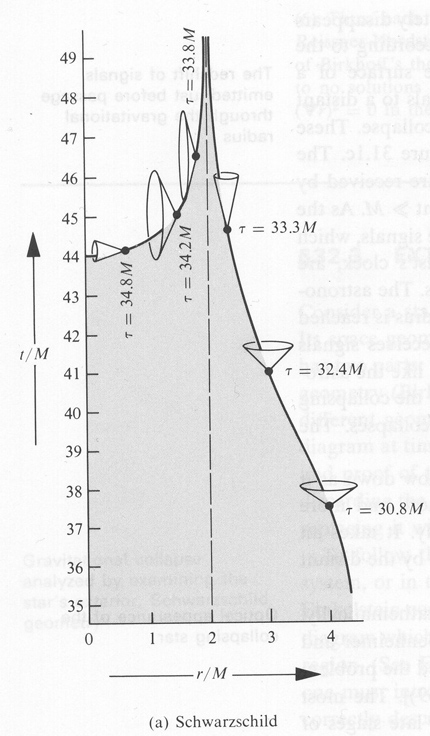
\includegraphics[width=0.6\textwidth]{figure/Schwarzschilddiagram.jpg}
  \caption[Coni di luce nello spazio-tempo di Schwarzschild, usando le
  coordinate di Schwarzschild]{Coni di luce nello spazio-tempo di Schwarzschild,
    usando le coordinate di Schwarzschild.  Immagine presa
    da~\textcite{misner:gravitation}}
  \label{fig:coni-schwarzschild}
\end{figure}
Supponiamo che il corpo che ha dato origine al buco nero sia collassato
completamente, cioè che la densità al suo interno sia nulla ovunque, tranne
eventualmente nella singolarità \(r = 0\).  In questo modo possiamo applicare la
soluzione di Schwarzschild delle equazioni di Einstein nel vuoto anche nella
regione \(0 < r < r_{\textup{S}}\).  Qui non sono presenti singolarità, ma
risulta
\begin{subequations}
  \begin{align}
    g_{00} &= -\biggl(1 - \frac{r_{\textup{S}}}{r}\biggr) > 0, \\
    g_{11} &= \biggl(1 - \frac{r_{\textup{S}}}{r}\biggr)^{-1} < 0.
  \end{align}
\end{subequations}
Osserviamo che i segni sono invertiti rispetto al solito: per \(r <
r_{\textup{S}}\) spazio e tempo si scambiano di ruolo, la coordinata \(t\)
diventa una coordinata ``spaziale'' e la coordinata \(r\) una coordinata
``temporale''.  In questo senso possiamo affermare che nella regione \(r <
r_{\textup{S}}\) la metrica, che dipende da \(r\), non è più stazionaria.  Il
fatto che la metrica sia stazionaria al di fuori di questa regione dipende dalla
scelta delle coordinate: è vero in coordinate di Schwarzschild, ma adottando
altre coordinate questo può non essere più vero.  A ogni modo, in qualsiasi
sistema di coordinate si verifica che la metrica è dipendente dal tempo per \(r
< r_{\textup{S}}\).  Nella figura~\ref{fig:coni-schwarzschild} sono riportati i
coni di luce nella geometria di Schwarzschild.

La singolarità in \(r = r_{\textup{S}}\) non è in realtà una singolarità fisica
ma piuttosto una \emph{singolarità spuria} o \emph{pseudosingolarità}, è una
patologia dovuta alle coordinate in uso.  È possibile eliminare questa
singolarità con un opportuno cambiamento di coordinate.  Un corpo che attraversa
la superficie \(r = r_{\textup{S}}\) non percepisce nessun cambiamento
particolare: le forze mareali diventano sempre più intense avvicinandosi al
raggio di Schwarzschild, ma rimangono comunque finite.  È solo in \(r = 0\) che
queste diventano infinite e solo qui, pertanto, è presente una reale singolarità
fisica.

\subsubsection{Altri sistemi di coordinate}
\label{sec:altre-coordinate}

Ci sono vari sistemi di coordinate nei quali la metrica di Schwarzschild rimane
regolare in \(r = r_{\textup{S}}\), a differenza delle coordinate di
Schwarzschild, tuttavia queste trasformazioni rendono la metrica dipendente
dalla coordinata temporale anche nella regione esterna alla superficie di
redshift infinito.

\begin{figure}
  \centering
  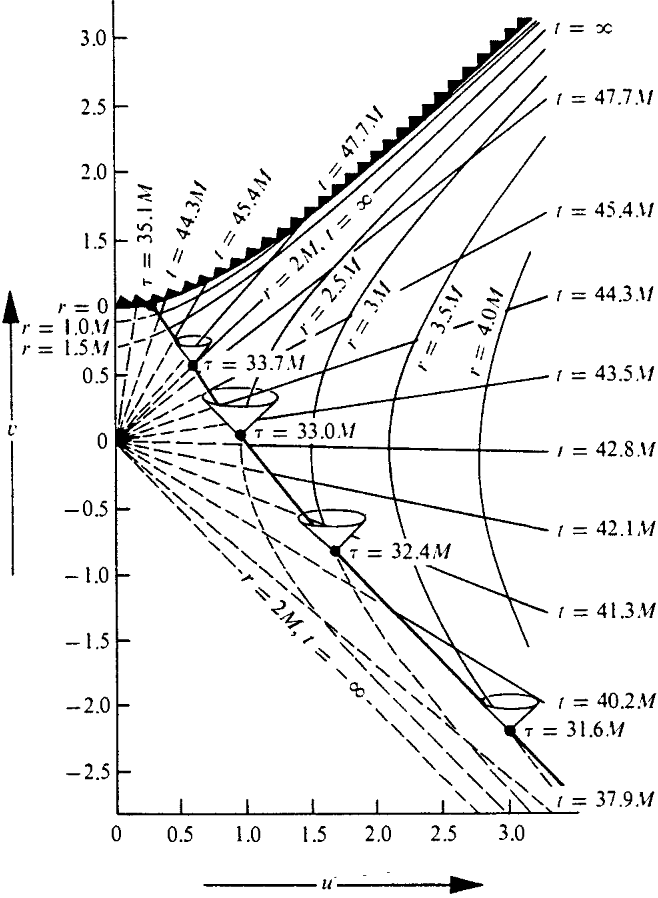
\includegraphics[width=0.7\textwidth]{figure/kruskal}
  \caption{Coni di luce nella geometria di Schwarzschild, usando le coordinate
    di Kruskal-Szekeres}
  \label{fig:coni-kruskal}
\end{figure}
Le coordinate di questo tipo più famose sono le \emph{coordinate di
  Kruskal-Szekeres}\index{coordinate!di Kruskal-Szekeres} \(u\) e \(v\) definite
in termini delle coordinate \(t\) e \(r\) di Schwarzschild dalle
relazioni~\parencites{1960PhRv..119.1743K}{1960PMatD...7..285S}
\begin{subequations}
  \allowdisplaybreaks{}
  \begin{align}
    v &=
    \begin{cases}
      \sqrt{1 - \dfrac{r}{r_{\textup{S}}}}\e^{r/2r_{\textup{S}}} \cosh
      \dfrac{t}{2r_{\textup{S}}}, & \text{per \(r < r_{\textup{S}}\),} \\[2.1ex]
      \sqrt{\dfrac{r}{r_{\textup{S}}} - 1}\e^{r/2r_{\textup{S}}} \sinh
      \dfrac{t}{2r_{\textup{S}}}, & \text{per \(r > r_{\textup{S}}\),}
    \end{cases} \\
    u &=
    \begin{cases}
      \sqrt{1 - \dfrac{r}{r_{\textup{S}}}}\e^{r/2r_{\textup{S}}} \sinh
      \dfrac{t}{2r_{\textup{S}}}, & \text{per \(r < r_{\textup{S}}\),} \\[2.1ex]
      \sqrt{\dfrac{r}{r_{\textup{S}}} - 1}\e^{r/2r_{\textup{S}}} \cosh
      \dfrac{t}{2r_{\textup{S}}}, & \text{per \(r > r_{\textup{S}}\),}
    \end{cases}
  \end{align}
\end{subequations}
La coordinata \(v\) è di tipo tempo e la coordinata \(u\) è di tipo spazio, le
coordinate angolari \(\theta\) e \(\phi\) sono le stesse delle coordinate di
Schwarzschild.  Le trasformazioni inverse per ricavare le coordinate \(t\) e
\(r\) di Schwarzschild sono
\begin{subequations}
  \allowdisplaybreaks{}
  \begin{gather}
    \label{eq:r-kruskal}
    \biggl(\frac{r}{r_{\textup{S}}} - 1\biggr)\e^{r/r_{\textup{S}}} = u^{2} -
                                                                      v^{2}, \\
    t =
        \begin{cases}
          2r_{\textup{S}}\tanh^{-1}\dfrac{u}{v} & \text{per \(r <
            r_{\textup{S}}\)}, \\[2.1ex]
          2r_{\textup{S}}\tanh^{-1}\dfrac{v}{u} & \text{per \(r >
            r_{\textup{S}}\)}.
        \end{cases}
  \end{gather}
\end{subequations}
Nelle coordinate di Kruskal-Szekeres, l'intervallo spazio-temporale con la
metrica di Schwarzschild si scrive come
\begin{equation}
  \dd\tau^{2} = \frac{4r_{\textup{S}}^{3}}{r}\e^{-r/r_{\textup{S}}}(\dd v^{2} -
  \dd u^{2}) - r^{2}\dd\theta^{2} - r^{2}\sin^{2}\theta\dd\phi^{2},
\end{equation}
in cui \(r\) è da intendersi come una funzione delle coordinate \(v\) e \(u\)
definita implicitamente dalla relazione~\eqref{eq:r-kruskal}.  Nella
figura~\ref{fig:coni-kruskal} sono rappresentati i coni di luce nello
spazio-tempo di Schwarzschild nelle coordinate di Kruskal-Szekeres.

\begin{figure}
  \centering
  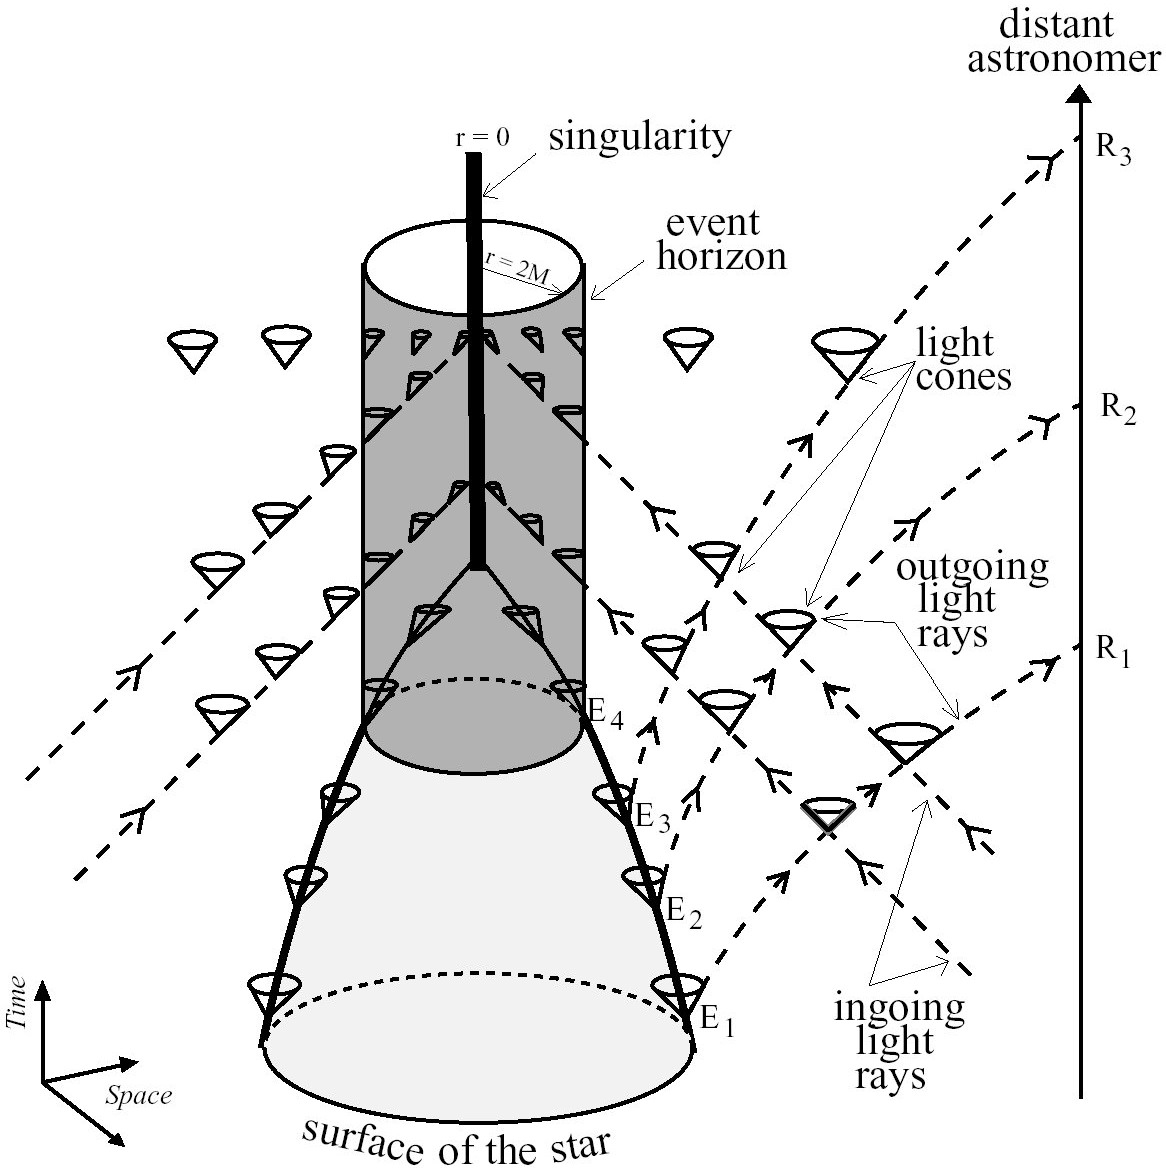
\includegraphics[width=0.5\textwidth]{figure/eddington}
  \caption{Coni di luce nella geometria di Schwarzschild, usando le coordinate
    di Eddington-Finkelstein}
  \label{fig:coni-eddington}
\end{figure}
Le \index{coordinate!di Eddington-Finkelstein}\emph{coordinate di
  Eddington-Finkelstein} sono una via di mezzo fra le coordinate di
Schwarzschild e le coordinate di Kruskal-Szekeres: la metrica risultante non
dipende dal tempo per \(r > r_{\textup{S}}\) e una delle due pseudosingolarità
in \(r = r_{\textup{S}}\) è rimossa.  Le coordinate di Eddington-Finkelstein
\(r\), \(\theta\) e \(\phi\) sono le stesse di Schwarzschild, mentre la
coordinata temporale \(\tilde{v}\) è definita
da~\parencites{1924Natur.113..192E}{1958PhRv..110..965F}
\begin{equation}
  \tilde{v} = t + r + r_{\textup{S}} \ln\abs*{\frac{r}{r_{\textup{S}}} - 1}.
\end{equation}
Con questa trasformazione, l'intervallo spazio-temporale della geometria di
Schwarzschild diventa
\begin{equation}
  \dd\tau^{2} = \biggl(1 - \frac{r_{\textup{S}}}{r}\biggr)\dd\tilde{v}^{2} -
  2\dd\tilde{v}\dd r - r^{2}\dd\theta^{2} - r^{2}\sin^{2}\theta\dd\phi^{2}.
\end{equation}
Nella parte spaziale della metrica non c'è più la pseudosingolarità in \(r =
r_{\textup{S}}\), che però rimane nella parte temporale.  Un inconveniente di
queste coordinate è che nella metrica sono introdotti dei termini non diagonali.
Nella figura~\ref{fig:coni-eddington} sono rappresentati i coni di luce nello
spazio-tempo di Schwarzschild adottando le coordinate di Eddington-Finkelstein.

\subsection{Buco nero rotante}
\label{sec:singolarita-kerr}

Anche un buco nero di Kerr ha una superficie di redshift infinito, individuata
dalla condizione \(g_{00} = 0\).  Dalla metrica~\eqref{eq:metrica-kerr} abbiamo
\begin{equation}
  0 = g_{00} = -\biggl(1 - \frac{r_{\textup{S}}r}{\Sigma}\biggr) = -\frac{r^{2}
    + a^{2}\cos^{2}\theta - 2 Mr}{r^{2} + a^{2}\cos^{2}\theta}
\end{equation}
da cui ricaviamo
\begin{equation}
  r_{\textup{E}}^{\pm} = M \pm \sqrt{M^{2} - a^{2}\cos^{2}\theta}.
\end{equation}
Pertanto, attorno a un buco nero rotante sono presenti due superfici distinte di
redshift infinito, non legate però ad alcuna singolarità fisica.  Come nel caso
del buco nero di Schwarzschild, sulla superficie in cui si annulla \(g_{00}\) in
metrica di Kerr una particella non può rimanere in quiete (con \(\dd r =
\dd\theta = \dd\phi = 0\)), solo un segnale luminoso emesso in direzione radiale
può raggiungere tale stato.  Nella regione compresa fra le due superfici di
redshift infinito \(g_{00}\) è positivo quindi la coordinata \(t\) è di tipo
``spazio'' e il fatto che la metrica sia indipendente da \(t\) non significa che
sia realmente indipendente dal tempo.

Dal calcolo dell'invariante quadratico di curvatura\footnote{Questa quantità è
  la \emph{norma di Hilbert-Schmidt} del tensore di Riemann.}
\(R^{\alpha\beta\gamma\delta}R_{\alpha\beta\gamma\delta}\) si scopre che l'unica
singolarità fisica, in cui l'invariante diverge, è presente in
(vedi~\textcite{2007arXiv0706.0622V}) \(\Sigma = r^{2} + a^{2}\cos^{2}\theta =
0\), cioè
\begin{subequations}
  \label{eq:singolarita-kerr}
  \begin{align}
    r &= 0, \\
    \theta &= \pi/2.
  \end{align}
\end{subequations}
Nelle coordinate di Boyer-Lindquist con \(a \neq 0\), \(r = 0\) non corrisponde,
in coordinate cartesiane \((x, y, z)\), a un punto ma a un disco.  Per esempio,
ricordando le trasformazioni~\eqref{eq:boyer-lindquist-debole} per un campo
debole, troviamo che le~\eqref{eq:singolarita-kerr} equivalgono alle condizioni
\begin{subequations}
  \begin{gather}
    x^{2} + y^{2} = a^{2}, \\
    z = 0.
  \end{gather}
\end{subequations}
Questa regione è un disco e nel caso del buco nero di Kerr si parla di
\emph{singolarità a disco} o \emph{singolarità ad anello} (\emph{disk
  singularity} o \emph{ring singularity} in inglese).  Nel limite \(a\to 0\) si
riottiene la singolarità puntuale di Schwarzschild \(x^{2} + y^{2} + z^{2} =
0\).

\section{Orizzonte degli eventi}
\label{sec:orizzonte-eventi}

\subsection{Buco nero non rotante}
\label{sec:orizzonte-schwarzschild}

Abbiamo visto che nella regione \(r < r_{\textup{S}}\) non ci sono dei
comportamenti locali patologici, tranne nella singolarità fisica \(r = 0\) dove
la curvatura e le forze mareali diventano infinite, ma adesso scopriremo che si
verificano dei fenomeni molto particolari di carattere globale.  In particolare,
troveremo che la regione \(r \leq r_{\textup{S}}\) è un buco nero, in base alla
definizione data a pagina~\pageref{definizione-buco-nero}.  Nessun tipo di
segnale può passare dalla regione \(r\leq r_{\textup{S}}\) alla regione \(r >
r_{\textup{S}}\).  Quindi, la superficie \(r = r_{\textup{S}}\) è il confine che
separa gli eventi che un osservatore esterno può vedere da quegli eventi che
rimarranno per sempre a lui inaccessibili, è l'orizzonte degli eventi di un buco
nero di Schwarzschild.

La velocità di un segnale luminoso che si propaga radialmente (quindi
\(\dd\theta = \dd\phi = 0\)) si ottiene calcolando \(\ltoder{r}{t}\) dopo aver
posto \(\dd\tau^{2} = 0\) nell'espressione~\eqref{eq:metrica-schwarzschild-bh}
dell'intervallo spazio-temporale della metrica di Schwarzschild
\begin{equation}
  \toder{r}{t} = \pm \biggl(1 - \frac{r_{\textup{S}}}{r}\biggr).
\end{equation}
Per \(r \to r_{\textup{S}}\), la velocità del segnale tende a \(0\).  Da qui
iniziamo a intuire che la superficie \(r = r_{\textup{S}}\) costituisce
l'orizzonte degli eventi di un buco nero non rotante.  L'analisi dei coni di
luce in coordinate di Schwarzschild, rappresentati nella
figura~\ref{fig:coni-schwarzschild}, aiuta a comprendere ciò che succede a un
segnale che attraversa dall'esterno l'orizzonte degli eventi.  Per \(r >
r_{\textup{S}}\) l'asse del cono, che indica la direzione del suo ``futuro'', è
parallelo all'asse \(t\), mentre nella regione \(r < r_{\textup{S}}\) è
parallelo all'asse \(r\).  Ogni segnale emesso a un dato evento può propagarsi
all'interno delle falde del cono luce di quell'evento: poiché per \(r <
r_{\textup{S}}\) i coni di luce sono orientati verso \(r = 0\), tutti i segnali
sono costretti a dirigersi inesorabilmente verso valori minori di \(r\), senza
la possibilità di tornare più indietro.  Osserviamo in particolare che
all'interno del buco nero niente può stare più fermo, ogni segnale dovrà essere
necessariamente in movimento.  Il bizzarro orientamento dei coni di luce
all'interno del buco nero riflette lo scambio di ruolo delle coordinate \(t\) e
\(r\) evidenziato nel paragrafo~\ref{sec:singolarita}.  Notiamo anche che in
questa regione è \(\ltoder{t}{r}\) che quantifica ciò che chiameremmo
``velocità'', il rapporto incrementale fra la coordinata spaziale e quella
temporale.

In un buco nero di Schwarzschild e orizzonte degli eventi coincidono, ma questo
non si verifica nel caso di altre soluzioni delle equazioni di Einstein, come
quella di Kerr, e adesso vedremo che non c'è alcuna ragione, in linea di
principio, per la quale queste due superfici debbano necessariamente coincidere.
Intanto iniziamo col notare che il fatto che su una superficie ci sia redshift
infinito, secondo un osservatore statico all'infinito, non impedisce di
comunicare attraverso questa superficie: può succedere che il redshift di una
sorgente di segnali situata all'interno della superficie di redshift infinito
sia, per un osservatore molto lontano, ridotto a un valore finito.  Inoltre il
redshift totale di un segnale dipende anche dalla velocità della sua sorgente e
l'effetto Doppler in alcuni casi può compensare interamente o in parte il
redshift gravitazionale.  Pertanto la superficie di redshift infinito è definita
in relazione a una specifica classe di sorgenti e ricevitori.  Invece, un
orizzonte degli eventi è una proprietà intrinseca dello spazio-tempo,
indipendentemente dallo stato di moto di sorgente e osservatore.  Tutti gli
osservatori esterni saranno d'accordo sul fatto che una certa superficie, \(r =
r_{\textup{S}}\) nel caso della geometria di Schwarzschild, costituisce un
orizzonte degli eventi dello spazio-tempo.

\subsection{Buco nero rotante}
\label{sec:orizzonte-kerr}

\begin{figure}
  \centering
  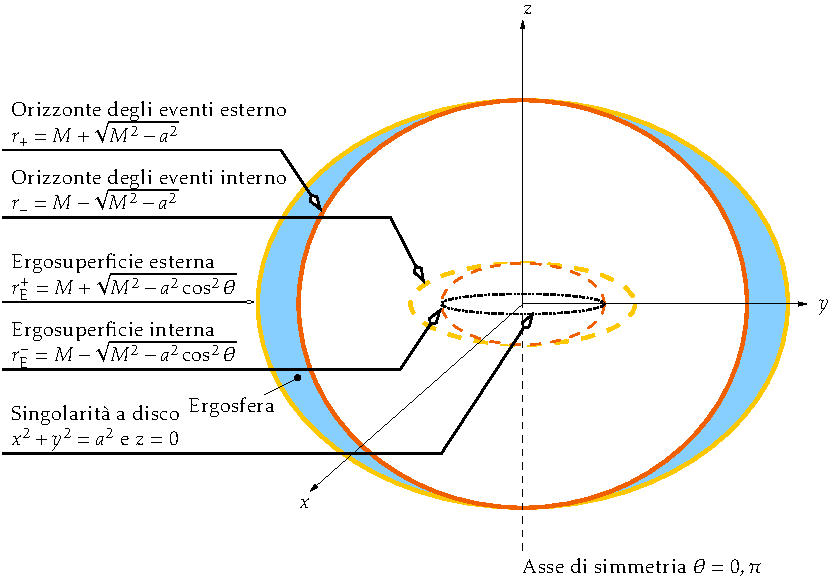
\includegraphics[width=\textwidth]{figure/kerr}
  \caption[Rappresentazione schematica della posizione degli orizzonti, delle
  ergosuperfici e della singolarità nella metrica di Kerr]{Rappresentazione
    schematica della posizione degli orizzonti, delle ergosuperfici e della
    singolarità nella metrica di Kerr.  Figura adattata
    da~\textcite{2007arXiv0706.0622V}}
  \label{fig:geometria-kerr}
\end{figure}
La posizione degli orizzonti degli eventi è individuata dalla condizione
\(\ltoder{r}{t} = 0\), per valori arbitrari di \(\dd\theta\) e \(\dd\phi\).
Ponendo l'intervallo spazio-temporale \(\dd\tau^{2}\) di
Kerr~\eqref{eq:metrica-kerr} uguale a \(0\) e risolvendo per
\((\ltoder{r}{t})^{2}\) si ottiene un'espressione un po' complicata, in cui però
si può prendere \(\Delta\) come fattore moltiplicativo globale.  Pertanto la
condizione \(\ltoder{r}{t} = 0\) è equivalente a
\begin{equation}
  \Delta = r^{2} - 2M + a^{2} = 0,
\end{equation}
da cui si trovano le due soluzioni
\begin{equation}
  r_{\pm} = M \pm \sqrt{M^{2} - a^{2}}.
\end{equation}
Sulle superfici \(r = r_{\pm}\) un segnale luminoso ha velocità nulla nella
direzione radiale e non può uscire da esse.  La superficie \(r = r_{+}\)
definisce il confine esterno del buco nero rotante, invece la superficie \(r =
r_{-}\) costituisce un confine più interno.  Notiamo che per \(\abs{a} < M\) il
buco nero ha due distinti orizzonti degli eventi, se \(\abs{a} = M\) ha un solo
orizzonte in \(r = M = r_{S}/2\), mentre per \(\abs{a} > M\) non c'è alcun
orizzonte.\footnote{In quest'ultimo caso la singolarità non è nascosta da un
  orizzonte degli eventi e si parla di \emph{singolarità nuda}.  Per \(\abs{a} >
  M\) non si ha neanche un buco nero vero e proprio dato che non c'è alcun
  orizzonte.  Sebbene le singolarità nude siano ammesse matematicamente dalla
  soluzione dell'equazione di Einstein, \textcite{1969NCimR...1..252P} ha
  congetturato che nelle reali condizioni fisiche in cui avviene il collasso
  gravitazionale di una massa non si verifichi mai la formazione di una
  singolarità nuda.  Questa ipotesi, ancora non dimostrata formalmente, è
  chiamata \emph{ipotesi del censore cosmico}.}  Nella metrica di Kerr è
evidente che superficie di redshift infinito e orizzonte degli eventi non
coincidono.  Nel limite di Schwarzschild \(a\to 0\) i due orizzonti si trovano
in \(r_{+} = 2M = r_{\textup{S}}\) e \(r_{-} = 0\).

Nella regione fra i due orizzonti risulta \(g_{11} < 0\) e quindi \(r\) è una
coordinata di tipo ``tempo''.  Come già osservato nel caso di Schwarzschild, in
questa regione la dipendenza da \(r\) della metrica comporta che questa sia
dinamica.  La regione compresa fra la superficie esterna di redshift infinito e
l'orizzonte esterno è chiamata \emph{ergosfera}.  L'ergosfera presenta un
particolare interesse perché, in base alla teoria non quantistica della
gravitazione, tutta la materia che entra in un buco nero è irrimediabilmente
persa, ma sembra non essere questo il caso dell'energia: un processo ideato
da~\textcite{1969NCimR...1..252P} permette di estrarre energia rotazionale da un
buco nero di Kerr sfruttando particelle che entrano ed escono dall'ergosfera.
Le principali caratteristiche dello spazio-tempo di Kerr sono illustrate nella
figura~\ref{fig:geometria-kerr}.

%%% Local Variables:
%%% mode: latex
%%% TeX-master: "../gravitazione"
%%% End:
